%=================================================================================================
%= = = = = = = = = = = = = = = = = = = = = = = = = = = = = = = = = = = = = = = = = = = = = = = = =
%=																								 =
%=							   >  >  INFORMAÇÕES DO DOCUMENTO  <  <								 =
%=																								 =
%= = = = = = = = = = = = = = = = = = = = = = = = = = = = = = = = = = = = = = = = = = = = = = = = =
%=================================================================================================

\documentclass[a4paper,10pt,compsoc]{IEEEtran}

\usepackage{cmap}											%-> Mapear caracteres especiais no PDF
\usepackage[T1]{fontenc}									%-> Selecao de códigos de fonte
\usepackage[utf8]{inputenc}									%-> Codificacao do documento
\usepackage{indentfirst}									%-> Indenta o primeiro parágrafo seção
\usepackage{color}											%-> Controle das cores
\usepackage{graphicx}										%-> Inclusão de gráficos
\usepackage{units}											%-> 
\usepackage[english,brazil]{babel}							%-> documento em Português e Inglês
\usepackage{bold-extra}										%-> 
\usepackage{eso-pic}										%-> 
\usepackage{geometry}										%-> 


%=================================================================================================
%= = = = = = = = = = = = = = = = = = = = = = = = = = = = = = = = = = = = = = = = = = = = = = = = =
%=																								 =
%=									 CONFIGURAÇÕES DO HYPERREF									 =
%=																								 =
%= = = = = = = = = = = = = = = = = = = = = = = = = = = = = = = = = = = = = = = = = = = = = = = = =
%=================================================================================================


\setlength{\columnsep}{6mm}									%-> Distância entre as colunas
\geometry{left=1.5cm,right=1.5cm,top=1.5cm,bottom=1.5cm}	%-> 























%=================================================================================================
%= = = = = = = = = = = = = = = = = = = = = = = = = = = = = = = = = = = = = = = = = = = = = = = = =
%=================================================================================================									%-> Setup
%%=================================================================================================
%= = = = = = = = = = = = = = = = = = = = = = = = = = = = = = = = = = = = = = = = = = = = = = = = =
%=																								 =
%=									 	CRIAÇÃO DE COMANDOS										 =
%=																								 =
%= = = = = = = = = = = = = = = = = = = = = = = = = = = = = = = = = = = = = = = = = = = = = = = = =
%=================================================================================================


% - INSTRUÇÕES: -------------------------------------
% -													-
% - Este ambiente é destinado à criação de novos	-
% - comandos que conferirão a este documento		-
% - novas funcionalidades.							-
% -													-
% ---------------------------------------------------


% COMANDOS DE INFORMAÇÕES GERAIS DO DOCUMENTO ====================================================


% INFORMAÇÕES GERAIS -----------------------------------------------------------------------------

\newcommand{\citarautor}[1]{\def\imprimircitarautor{#1}}	%-> Comando para Citação de Autor

\newcommand{\instituto}[1]{\def\imprimirinstituto{#1}}		%-> Comando para Instituto

\newcommand{\faculdade}[1]{\def\imprimirfaculdade{#1}}		%-> Comando para Faculdade

\newcommand{\curso}[1]{\def\imprimircurso{#1}}				%-> Comando para Curso

\newcommand{\disciplina}[1]{\def\imprimirdisciplina{#1}}	%-> Comando para Grau Acadêmico


\newcommand{\local}[1]{\def\imprimirlocal{#1}}				%-> Comando para Grau Acadêmico

\newcommand{\data}[1]{\def\imprimirdata{#1}}				%-> Comando para Grau Acadêmico


% ORIENTADOR E COORIENTADOR - TITULAÇÃO ACADÊMICA ------------------------------------------------


%=================================================================================================
%= = = = = = = = = = = = = = = = = = = = = = = = = = = = = = = = = = = = = = = = = = = = = = = = =
%=================================================================================================								%-> Comandos para novas funcionalidades
%%=================================================================================================
%= = = = = = = = = = = = = = = = = = = = = = = = = = = = = = = = = = = = = = = = = = = = = = = = =
%=																								 =
%=							   >  >  INFORMAÇÕES DO DOCUMENTO  <  <								 =
%=																								 =
%= = = = = = = = = = = = = = = = = = = = = = = = = = = = = = = = = = = = = = = = = = = = = = = = =
%=================================================================================================


% - INSTRUÇÕES: -------------------------------------
% -													-
% - Preencha as informações gerais do documento	nos -
% - respectivos campos indicados.					-
% -													-
% ---------------------------------------------------



% TÍTULO =========================================================================================

\title{\textsf{
\bfseries \Huge Uso de Redes Neurais Artificiais na Previsão\\ 
do Consumo de Energia}}


% AUTORES =========================================================================================












%=================================================================================================
%= = = = = = = = = = = = = = = = = = = = = = = = = = = = = = = = = = = = = = = = = = = = = = = = =
%=================================================================================================							%-> Informações Gerais do Documento


\begin{document}

% ELEMENTOS PRÉ-TEXTUAIS =========================================================================

\twocolumn[
\begin{@twocolumnfalse}

\begin{center}
%=================================================================================================
%= = = = = = = = = = = = = = = = = = = = = = = = = = = = = = = = = = = = = = = = = = = = = = = = =
%=																								 =
%=							   		   >  >  CABEÇALHO  <  <									 =
%=																								 =
%= = = = = = = = = = = = = = = = = = = = = = = = = = = = = = = = = = = = = = = = = = = = = = = = =
%=================================================================================================


% - INSTRUÇÕES: -------------------------------------
% -													-
% - Preencha as informações gerais do documento	nos -
% - respectivos campos indicados.					-
% -													-
% ---------------------------------------------------


\begin{center}

% DADOS PESSOAIS =================================================================================

\vspace*{2 cm}

\textsf{\bfseries 
\huge Uso de Estruturas Competitiva de Redes Neurais \\[3 mm]
Auto Associativas na Classificação
de Tipos de Vinho}


% AUTORIA ========================================================================================

\vspace*{1.5 cm}

	\begin{large}
Luiz Henrique P. Assunção$^{1}$ e
Paulo Vinícius Nobre Normando$^{2}$
	\end{large} \\[1.7 mm]


% DADOS DA INSTITUIÇÃO ===========================================================================

	\begin{small}
$^{1\ 2}$Faculdade de Engenharia Elétrica e Biomédica, Universidade Federal do Pará, \\[1 mm]
Av. Augusto Correa 01, Belém, Pará 66075-090, Brasil \\[7 mm]


% AUTORIA ========================================================================================

Autor Correspondente$^{1}$: luiz.heinrich@live.com	\\[1 mm]
Autor Correspondente$^{2}$: paulonormando@gmail.com

	\end{small}

\end{center}
 

%=================================================================================================
%= = = = = = = = = = = = = = = = = = = = = = = = = = = = = = = = = = = = = = = = = = = = = = = = =
%=================================================================================================			%->	Capa
%=================================================================================================
%=							       		      SUMÁRIO											 =
%=================================================================================================



\begin{center}


\begin{minipage}[c][5cm]{15cm}		%-> [Altura] [Largura]
	
\begin{abstract}

\noindent
Nós estudamos duas arquiteturas de Redes Neurais Artificiais para um problema de classificação de três tipos de vinhos, com a finalidade de comparar a acurácia das duas redes no problema de classificação proposto. A primeira arquitetura estudada é uma rede mais simples, a Perceptron de Multiplas Camadas (MPL), e já a segunda é uma Estrutura Competitiva de MPL Auto Associativa. O banco de dados é composto de 178 instâncias de 13 parâmetros das 3 classes de vinho. Primeiramente, nós normalizamos as entradas do banco de dados e implementamos os algorítimos das duas arquiteturas no software MATLAB. Como resultado, podemos identificar através do estudo do erro que a arquitetura de Competição Auto Associativa obteve um melhor desempenho para a classificação do que uma rede Perceptron de Múltiplas Camadas.
\\[1 mm]
\textbf{Palavras-chave}: Redes Neurais Artificiais. Redes Auto Associativas. Vinho. MATLAB.

\end{abstract}

\end{minipage}


\end{center} \vspace*{0.5 cm}

					%->	Resumo
\end{center}

\end{@twocolumnfalse}]


% ELEMENTOS TEXTUAIS =============================================================================

%=================================================================================================
%=							       		    INTRODUÇÃO							     			 =
%=================================================================================================

\section{Introdução} \label{introducao}

As Redes Neurais Artificiais (RNA) são modelos matemáticos-computacionais que visam simular o comportamento e arquitetura de um neurônio biológico. Essa característica confere a uma RNA a capacidade de reconhecer e classificar padrões a partir de um modelo de aprendizagem baseado no aprendizado humano \cite{kovacs2002redes}.

Fazendo o uso de RNAs, o presente artigo trata do problema de classificação de Vinho. E este, é um conjunto de dados multivariado introduzido por \textit{M. Florina}, o qual consiste em 178 amostras de 13 quesitos do vinho avaliado, pertencentes às três classes de vinho.

Estes dados são os resultados de uma análise química de vinhos cultivados na mesma região na Itália, no entanto, derivados de três diferentes cultivares. A análise determinou as quantidades de 13 constituintes encontrados em cada um dos três tipos de vinhos \cite{fraley2007model}.

Desta forma, com base na combinação dessas 13 características, é possível classificar o tipo de vinho com base nas 178 amostras.

\subsection{Metodologia}

Para o fim proposto, foi usado o Software Matlab (R2018B), com o uso da toolbox de redes neurais.


\subsection{Objetivos}

Como objetivo geral, este trabalho implementa duas arquiteturas de Redes Neurais Artificiais para a classificação de três classes de vinho a partir dos 13 parâmetros de entrada. A primeira arquitetura é uma RNA de Múltiplas Camadas (MLP) e a segunda, a uma MLP com estrutura Competitiva Auto Associativa.

Enquanto que o objetivo específico é averiguar e comparar a melhor arquitetura de rede para o problema de classificação proposto.


\subsection{Organização do Trabalho}

Este artigo está organizado como se segue. Na Seção \ref{revisaobibliografica} é feita uma revisão bibliográfica sobre Redes Neurais. Logo após, na Seção \ref{baseDados}, é apresentada a base de dados estudada neste artigo. Na Seção \ref{desenvolvimentoMLP} e na Seção \ref{desenvolvimentoAuto}, são apresentadas as arquiteturas das redes propostas, bem como por quais metodologias este trabalho se orienta. Os resultados são apresentados no Seção \ref{resultados}. Na Seção \ref{consideracoesFinais}, as considerações finais desde trabalho.					%-> Introdução
\section{Revisão Bibliográfica} \label{revisaobibliografica}

Redes Neurais Artificiais são técnicas computacionais que apresentam um modelo matemático inspirado na estrutura neural de organismos inteligentes e que adquirem conhecimento através da experiência. A arquitetura base de rede neural estudada neste artigo é a Perceptron de Múltiplas Camadas (do inglês, Multilayer Perceptron, ou apenas MLP).

\subsection{Perceptrom de Multiplas Camadas}

Uma rede MLP consiste em pelo menos três camadas: uma camada de entrada, uma camada oculta e uma camada de saída. O MLP utiliza uma técnica de aprendizado supervisionada chamada \textit{backpropagation} para o treinamento.

\begin{figure}[H]

\centering % para centralizarmos a figura
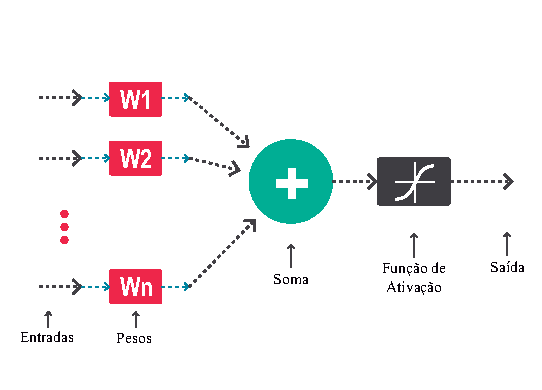
\includegraphics{04-Figuras/Arquitetura}

\caption{Arquitetura de uma rede MLP}

\label{figura:arquitetura}

\end{figure}

A rede é alimentada pela camada de entrada, de maneira que as entradas serão ponderadas por pesos e, logo em seguida, serão somados de submetidos a uma função de ativação (na camada intermediária). Por fim, após este processamento, haverá uma resposta na camada de saída da rede, como ilustra a fig. \ref{figura:arquitetura}.



\subsection{Algoritmo Backpropagation}


Quando verifica-se a resposta na camada de saída de uma MLP, podemos estimar o grau de acerto da rede. Portanto, há um valor esperado (e conhecido) para a resposta da rede durante a fase de treinamento. Logo, podemos extrair o erro dessa rede. O algoritmo \textit{backpropagation} visa realimentar o erro nas entradas com o objetivo de minimizá-lo ao máximo. Essa característica é chamada de retropropagação do erro.

\subsection{Estrutura Competitiva Auto Associativa}

Maecenas ipsum velit, consectetuer eu, lobortis ut, dictum at, dui. In rutrum. Sed ac dolor sit amet purus malesuada congue. In laoreet, magna id viverra tincidunt, sem odio bibendum justo, vel imperdiet sapien wisi sed libero. Suspendisse sagittis ultrices augue. Mauris metus. Nunc dapibus tortor vel mi dapibus sollicitudin. Etiam posuere lacus quis dolor. Praesent id justo in neque elementum ultrices. Class aptent taciti sociosqu ad litora torquent per conubia nostra, per inceptos hymenaeos. In convallis. Fusce suscipit libero eget elit. Praesent vitae arcu tempor neque lacinia pretium. Morbi imperdiet, mauris ac auctor dictum, nisl ligula egestas nulla, et sollicitudin sem purus in lacus.



Aenean placerat. In vulputate urna eu arcu. Aliquam erat volutpat. Suspendisse potenti. Morbi mattis felis at nunc. Duis viverra diam non justo. In nisl. Nullam sit amet magna in magna gravida vehicula. Mauris tincidunt sem sed arcu. Nunc posuere. Nullam lectus justo, vulputate eget, mollis sed, tempor sed, magna. Cum sociis natoque penatibus et magnis dis parturient montes, nascetur ridiculus mus. Etiam neque. Curabitur ligula sapien, pulvinar a, vestibulum quis, facilisis vel, sapien. Nullam eget nisl. Donec vitae arcu.

Morbi a metus. Phasellus enim erat, vestibulum vel, aliquam a, posuere eu, velit. Nullam sapien sem, ornare ac, nonummy non, lobortis a, enim. Nunc tincidunt ante vitae massa. Duis ante orci, molestie vitae, vehicula venenatis, tincidunt ac, pede. Nulla accumsan, elit sit amet varius semper, nulla mauris mollis quam, tempor suscipit diam nulla vel leo. Etiam commodo dui eget wisi. Donec iaculis gravida nulla. Donec quis nibh at felis congue commodo. Etiam bibendum elit eget erat.

Nam quis nulla. Integer malesuada. In in enim a arcu imperdiet malesuada. Sed vel lectus. Donec odio urna, tempus molestie, porttitor ut, iaculis quis, sem. Phasellus rhoncus. Aenean id metus id velit ullamcorper pulvinar. Vestibulum fermentum tortor id mi. Pellentesque ipsum. Nulla non arcu lacinia neque faucibus fringilla. Nulla non lectus sed nisl molestie malesuada. Proin in tellus sit amet nibh dignissim sagittis. Vivamus luctus egestas leo. Maecenas sollicitudin. Nullam rhoncus aliquam metus. Etiam egestas wisi a erat.


%=================================================================================================
%=================================================================================================

\section{Base de Dados} \label{baseDados}

A base de dados tratada neste trabalho é referente a 13 parâmetros (características) de três classes de vinho, onde totaliza 178 instâncias de dados coletados.

Das 178 instâncias 59 pertencem à classe 1, 71 pertencem à classe 2 e 48 à classe 3.



%=================================================================================================
%=================================================================================================


\section{Desenvolvimento da Rede MLP} \label{desenvolvimentoMLP}

A rede MLP foi implementada utilizando 13 neurônio na camada de entrada, 5 neurônio na camada intermediária e um neurônio na camada de saída.

A topologia da rede foi escolhida variando-se o número de neurônios na camada intermediária e fazendo um estudo sobre o erro médio quadrático (do inglês, MSE) e o número de erros na classificação.





\begin{table}[H]
\centering
\caption{Melhor topologia MLP}
\resizebox{\columnwidth}{!}{%
\begin{tabular}{ccc}
\hline
NEURÔNIOS & MSE                & ERROS \\ \hline
1         & 0.0705937829921329 & 3     \\
3         & 0.0630764717369302 & 2     \\
5         & 0.0157501702325207 & 1     \\
10        & 0.0779010995153948 & 1     \\
20        & 0.0883763713087734 & 2     \\
40        & 0.155451160809213  & 6     \\
80        & 0.158974910948916  & 5     \\ \hline
\end{tabular}%
}

\label{tabela:MLP_MSE}

\end{table}

							%->	Tabela 01

A tabela \ref{tabela:MLP_MSE} mostra o desempenho de cada topologia de rede MPL. Observa-se que o melhor desempenho foi obtido pela rede com 5 neurônios na camada intermediária, pois apresentou o menor erro médio quadrático e o menor número de erros na classificação.


\subsection{Arquitetura MLP}

\begin{figure}[H]

\centering % para centralizarmos a figura
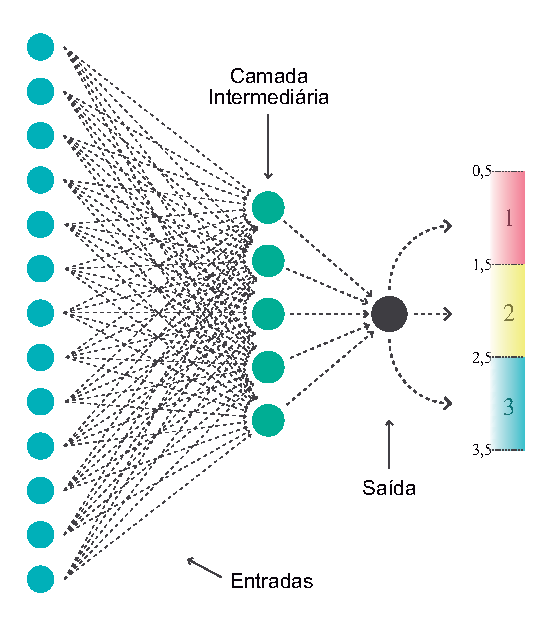
\includegraphics{04-Figuras/Arquitetura-MPL}

\caption{Arquitetura da rede MLP}

\label{figura:arquiteturaMPL}

\end{figure}

Após a escolha da topologia de rede MLP, 



\subsection{Parâmetros de Classificação}



A resposta da rede MLP foi definida em intervalos de abrangência. De 0,5 a 1,5, consideramos como pertencentes à classe 1. Os valores entre 1,5 a 2,5, são os da classe 2. Para a classe 3, foi definido o intervalo de 2,5 a 3,5.

%=================================================================================================
%=================================================================================================

\section{Desenvolvimento da Rede Competitiva Auto Associativa} \label{desenvolvimentoAuto}

A rede competitiva auto associativa é projetada sendo três redes, uma para cada classe, que serão treinadas para se especializarem na classe a qual elas representam. Assim, as três redes formam uma estrutura única de competição.


\subsection{Arquitetura}

A rede competitiva auto associativa foi implementada com 13 camadas de entrada e saída, sendo os seus argumentos os mesmos, e com 5 neurônios na camada intermediária, como mostra a fig. \ref{figura:arquiteturaAuto}.

\begin{figure}[H]

\centering % para centralizarmos a figura
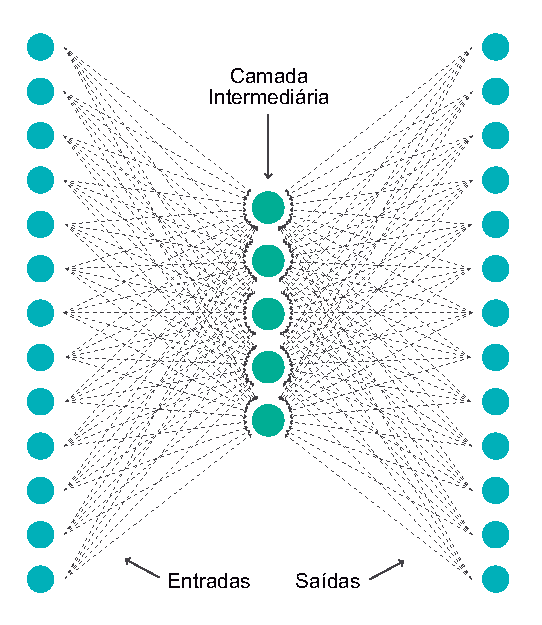
\includegraphics{04-Figuras/Arquitetura-AutoAssociativa}

\caption{Arquitetura da rede Competitiva Auto Associativa}

\label{figura:arquiteturaAuto}

\end{figure}			%-> Desenvolvimento
\section{Resultados} \label{resultados}

A mesma base de teste (sendo 10 de cada classe, totalizando 30) foi usada para verificar tanto o desempenho das 3 redes que compõe a auto associativa quanto da rede MLP.

O parâmetro de comparação foi o erro médio quadrático (MSE) obtido no desempenho das redes.


\subsection{Desempenho da Rede MLP}

A rede MLP apresentou um desempenho bom, tendo em vista que houve apenas 1 erro na classificação.

\begin{figure}[H]

\centering % para centralizarmos a figura
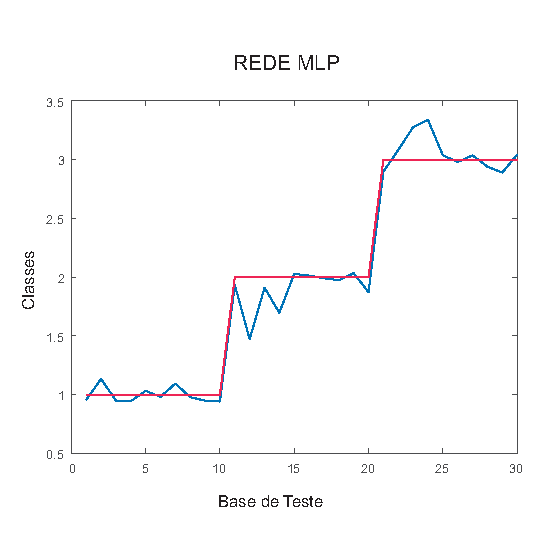
\includegraphics{04-Figuras/SAIDA_MLP}

\caption{Saída da rede MLP}

\label{figura:saidaMLP}

\end{figure}

A fig. \ref{figura:saidaMLP} mostra o desempenho da rede MLP, onde em azul é a saída da rede e em vermelho, a saída desejada.


\subsection{Desempenho da Rede Auto Associativa}

Considerando toda a base de teste (30 instâncias), as três redes que compõe a estrutura competitiva auto associativa apresentaram resultados bem interessantes para as classes nas quais elas são especializadas. No entanto, elas apresentaram erros consideráveis para as instâncias da base de teste pertencente às outras classes (o que de certa forma é esperado).


\subsubsection{Desempenho da Rede 1}

A fig. \ref{figura:rede1} mostra o desempenho da rede 1, que é especializada na classe 1.

\begin{figure}[H]

\centering % para centralizarmos a figura
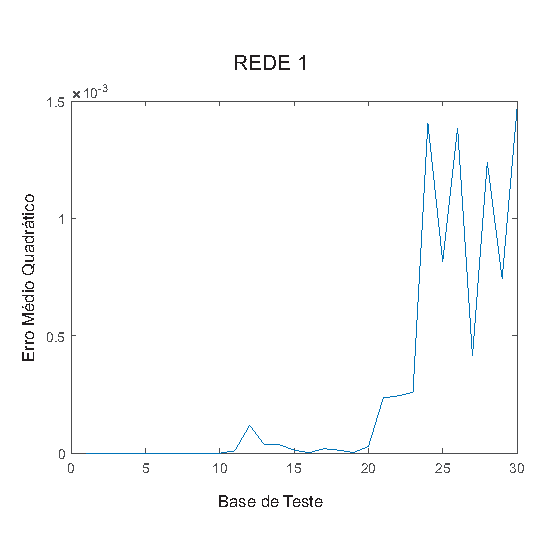
\includegraphics{04-Figuras/MSE_DesempenhoNet1}

\caption{Desempenho da rede 1}

\label{figura:rede1}

\end{figure}

Observa-se que o erro médio quadrático é extremamente baixo para a base de dados de 1 a 10 (que corresponde à classe 1) e bastante significativo entre 11 a 30, que são instâncias pertencentes às classes 2 e 3.

\subsubsection{Desempenho da Rede 2}

Na rede 2, o padrão de comportamento da rede 1 se repetiu. Observa-se que de 1 a 10 o MSE é acentuado, sendo extremamente baixo de 11 a 20 (instâncias pertencentes à classe 2), e novamente alto de 21 a 30, como mostrado na fig. \ref{figura:rede2}.

\begin{figure}[H]

\centering % para centralizarmos a figura
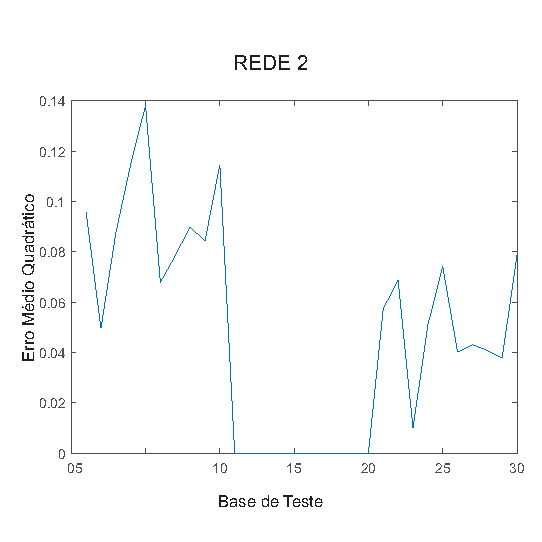
\includegraphics{04-Figuras/MSE_DesempenhoNet2}

\caption{Desempenho da rede 2}

\label{figura:rede2}

\end{figure}

\subsubsection{Desempenho da Rede 3}

Seguindo a tendência de comportamento, a rede 3 apresentou um alto valor do MSE para as instâncias de 1 a 20 (pertencentes às classes 1 e 2), bem como um erro muito baixo para as instâncias da classe 3, onde a rede 3 é especializada, de 21 a 30.

\begin{figure}[H]

\centering % para centralizarmos a figura
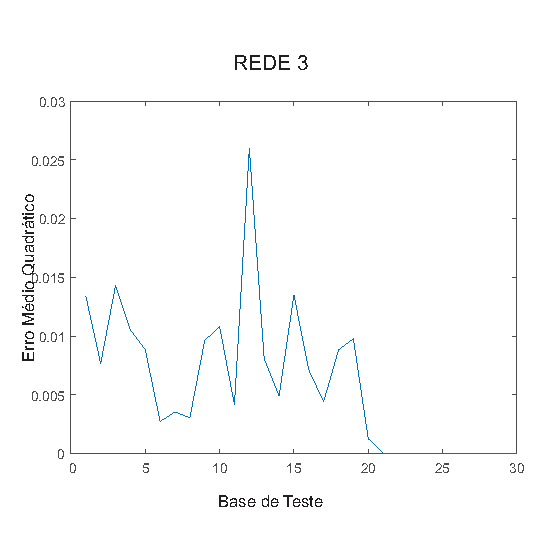
\includegraphics{04-Figuras/MSE_DesempenhoNet3}

\caption{Desempenho da rede 3}

\label{figura:rede3}

\end{figure}



\subsection{Comparação Rede MLP X Rede Auto Associativa}

Varius erat fames feugiat pellentesque eros laoreet lacinia integer condimentum sed vulputate, integer condimentum eleifend maecenas dapibus viverra nunc rhoncus eros. volutpat consectetur dictum purus etiam augue ipsum litora consectetur commodo mi, commodo est cursus sem ac cubilia conubia in at. ligula fermentum nisl erat sed posuere ac fusce sociosqu, porttitor vulputate tellus platea duis tristique tellus. vehicula varius pellentesque nam sapien aptent, et vivamus eget turpis ac, sit bibendum eros varius. venenatis ultrices dui sollicitudin aliquam pellentesque sagittis elit sociosqu ut, lorem consectetur adipiscing eu elementum ipsum nullam eros, egestas ligula dapibus congue est ornare vitae hendrerit.

Tabela de comparação					%-> Resultados
\section{Considerações Finais} \label{consideracoesFinais}

\subsection{Discussão}

A proposta de uma Rede Neural especializada em cada classe confere um desempenho muito bom em problemas de classificação. Assim, em uma estrutura Competitiva Auto Associativa, o que se tem são três redes dedicadas a cada uma das classes. Diferentemente da Rede MPL, onde uma só rede tem o dever de classificar as três classes de vinho estudada.


\subsection{Conclusão}

As redes com estrutura Competitiva Auto Associativa demonstraram um desempenho significativamente maior frente à rede MPL. Portanto, as redes Auto Associativas têm uma grande confiabilidade para problemas de classificação.


\subsection{Trabalhos Atuais e Sugestões Para Trabalhos Futuros}

Dapibus gravida tristique sodales purus condimentum porttitor, aliquam vulputate condimentum donec sapien justo praesent, sociosqu pellentesque dictum eros auctor. odio amet sem pretium eros facilisis curabitur velit tempus sapien, sodales praesent rutrum interdum tincidunt habitant euismod augue, tristique vehicula tempus molestie at quisque erat potenti. lacinia pulvinar class dictumst suspendisse eget etiam, molestie lectus class aenean purus eros primis, quam purus lectus viverra est. ante eget pretium lacus torquent cras ullamcorper neque, elit platea diam nulla potenti class auctor lectus, tempor dapibus a justo aptent rhoncus. praesent aliquet purus felis nostra pellentesque odio quisque praesent porttitor, curae maecenas placerat nostra maecenas erat ac tristique, iaculis porttitor habitant aptent suscipit posuere accumsan curabitur. 		%-> Considerações Finais


% ELEMENTOS PÓS-TEXTUAIS =========================================================================

% use section* for acknowledgment
%\section*{Acknowledgment}
			%-> Agradecimentos
%\appendices
\section{Proof of the First Zonklar Equation}
Appendix one text goes here.

% you can choose not to have a title for an appendix
% if you want by leaving the argument blank
\section{}
Appendix two text goes here.

					%-> Anexo
%=================================================================================================
%=							       		    REFERÊNCIAS											 =
%=================================================================================================


%\section{Referências Bibliográficas}



\bibliographystyle{ieeetr}
\bibliography{Bibliografia}			%-> Referências


%=================================================================================================

\end{document}